%!TEX root = ../thesis_rui_almeida.tex
%%%%%%%%%%%%%%%%%%%%%%%%%%%%%%%%%%%%%%%%%%%%%%%%%%%%%%%%%%%%%%%%%%%%
%% 3_methods.tex
%% Rui V. Almeida's thesis file
%%
%% This chapter contains the methods presentations and discussion
%%%%%%%%%%%%%%%%%%%%%%%%%%%%%%%%%%%%%%%%%%%%%%%%%%%%%%%%%%%%%%%%%%%%
\chapter{Methods}
\label{cha:methods}

Macroscopically, the approach to the \gls{RQ} was conducted by working
with two hypothesis:
\begin{description}
    \item[First Hypothesis:] The definition of a particular set of
        algorithmically defined projections in such a manner that they
        might be used for tomographic reconstruction of column densities
        of trace gases in the atmosphere, in a given \gls{ROI};
    \item[Second Hypothesis:] We can retrieve the column density for a
        given trace gas (or set of trace gases) between two points by
        performing a spectral measurement in both of these points in the
        same direction and subtracting them one from the other.
\end{description}

To test the first hypothesis, I have used a number of computational
methods to define and create projection and backprojection matricial
operators, resulting in a dedicated simulation software tool that proves
without a doubt that the devised projection gathering strategy is able
to produce projection information in sufficient quantity as to perform
tomographic reconstruction. This procedure is detailed in
Section~\ref{sec:tomosim}. 

The second hypothesis was experimentally tested, by the conduction of a
number of field experiments designed to determine the validity of
measurement hypothesis with the equipments to which I have current
access. The experiment and the protocol that was followed is detailed in
Section~\ref{sec:the_experiment}.

\section{Tomosim}%
\label{sec:tomosim}

Tomosim was the (somewhat unoriginal) name given to the tomographic
simulation software tool that was designed and built as part of this
project. It was created to tackle the trajectory-related hypothesis,
briefly described in this chapter's introduction.

The final system must be able to gather projection information by
reading spectral information, in this case the \gls{DOAS}-retrieved
column density for an atmospheric trace gas (or several) from a set of
predetermined directions. In "normal" tomographic \gls{DOAS}
application, these directions are fixed and depend on the experiment
infrastructure's geometry (see Section~\ref{sec:doas_tomography}). One
of the main novelties that I am trying to create with this project is a
very high degree of geometric freedom. A mobile system has no custom
infrastructure, and therefore has no fixed positions to which it is
tied. Instead its ability measure and monitor its atmospheric
surroundings relies on its movement. 

A ground-based mobile \gls{DOAS}-tomography system would have too strong
a dependency on open spaces and the topography of its \gls{ROI} to be
useful in any \textit{real world} scenario. A much more interesting and
feasible approach would be to use some kind of flying machine that could
carry spectroscopic equipment, and that could be programmed to fly in a
precise manner. Fortunately, current day technology provides a very
strong immediate candidate: a \gls{UAV} of the n-copter type, such as
the one in Figure~\ref{fig:an_hexacopter}\todo{image citation}.

\begin{figure}[htpb]
    \centering
    \missingfigure{An image of an hexacopter in flight.}
    \caption{Hexacopter in flight. Taken from laksjdlaksjd}
    \label{fig:an_hexacopter}
\end{figure}

A natural choice as it may seem as means for the measurements I am
describing in this document, its programming is almost (if not more) as
important as the hardware itself. The vehicle must be programmed to
describe a very precise (taking into account the type of operation we
are proposing) trajectory. In flight, the drone should be able to carry
and point an optical system towards any direction and in a short time.
Said optical system should be attached to a computer-controlled
spectrometer. This would allow the whole system to determine target
trace gas concentration on demand and programmatically.

The programmed trajectory should make use of these capabilities and
gather enough information for tomographic reconstruction. This also
means that the trajectory must be comprised of a sufficient number of
spectral projection acquisition \emph{opportunities}.

Of the several geometries that are described in the literature for
tomographic reconstructions, the one that seemed to be more promising in
terms of the balance between reconstruction complexity and the
information / flight time ratio was the fanbeam assembly (described in
Section~\ref{sec:tomographic_algorithms_and_reconstruction_techniques}).
It was the feasibility of this trajectory for the proposed purposes that
this simulation aimed to prove.

In essence, the drone's trajectory (illustrated in
Figure~\ref{fig:illustriated_trajectory_and_fanbeam_formation}) is a
horizontal circle which is parametrised to be at a certain height and to
have a certain diameter.  Both of these dimensions are set at experiment
/ measurement time. The drone stops on this circle at regular angular
intervals, say $\alpha$ degrees. Each one of these stops (360 / $\alpha$
stops) will generate a fanbeam projection, by pointing the optical
system inwards (with respect to the circular macro-trajectory) and
performing a series of spectroscopic measurements in different
directions and also at regular intervals, say $\gamma$ degrees. The
particular case in which $\alpha = \gamma$ is very interesting, because
it then opens the possibility for resorting the fanbeams into parallel
virtual-projections that are much easier to reconstruct tomographically,
as introduced in
Section~\ref{sec:tomographic_algorithms_and_reconstruction_techniques}.  

\begin{figure}[htpb]
    \centering
    \missingfigure{}
    \caption{Illustration of the projection gathering algorithm based on
    fanbeam assembly of information. On the left the circle which
    constitutes the general trajectory of the drone. On the right the
    gymbal points the optical system towards different directions, forming
    what can be seen as a fan.}
    \label{fig:illustriated_trajectory_and_fanbeam_formation}
\end{figure}



\section{The Experiment}%
\label{sec:the_experiment}








\section{Section Objectives}%
\label{sec:section_objectives}

\begin{itemize}
    \item Summarise, explain and recount how the question was answered;
    \item Discuss the previous point in details;
    \item Why are techniques relevant;
    \item How were the techniques used;
\end{itemize}

\section{Questions the readers should be able to answer once they've
read the section}%
\label{sec:questions_the_readers_should_be_able_to_answer_once_they_ve_read_the_section}
\begin{itemize}
    \item What are the results;
    \item How do the findings relate to previous studies;
    \item Was there anything surprising that did not go as planned;
    \item Why the presented conclusion have been reached;
    \item Explain results;
\end{itemize}


\section{How was the question answered?}%
\label{sec:how_was_the_question_answered_}
\textbf{Question}

How to design a miniaturised tomographic atmosphere monitoring system
based on DOAS?

\textbf{How was the question addressed?}

\begin{description}
    \item[Projection-based hypothesis:]first step was to design an
        information gathering approach. Ours was based on the definition
        of a particular trajectory for the measurement device. This had
        to be validated in computational and mathematical sense;
    \item[Measurement based hypothesis:] although it is clearly implied
        by Lambertian theory, there is no literature that I know of that
        points to the fact that my measurements are correct. Therefore,
        the assumption that we can measure columns densities between two
        points sequentially must be tested;
\end{description}

\section{Detailed presentation of projection-based hypothesis}%
\label{sec:detailed_presentation_of_projection_based_hypothesis}

\begin{description}
    \item[Hypothesis:]
        \begin{itemize}
            \item A tomographic atmospheric measurement entails
                capturing projections in many different angles;
            \item The typical atmospheric tomographic DOAS application
                uses serveral tens of projections for reconstruction;
            \item A drone moving in a circular trajectory would be able
                to capture an array of fan-beam projections with a
                specially motorised spectroscopic assembly;
            \item In theory, this would be sufficient for
                reconstruction;
            \item For simplicity, in this application we use the
                re-sorting reconstruction algorithm, which applies the
                FBP algorithm to a synthetically created parallel beam
                sinogram;
        \end{itemize}
    \item[How is the trajectory defined:\\]
        \begin{itemize}
            \item circular;
            \item one stop at each $\alpha$ degrees. At each one:
                \begin{itemize}
                    \item gymbal points to a number of directions
                        (parameter) at regular intervals (parameter),
                        taking one measurement at a time;
                \end{itemize}
            \item on a second moment, the drone moves to the entry
                points of the rays that have been capturesd by the
                equipment, taking a measurement at each one, in the same
                direction;
            \item use the measurement hypothesis to determine the
                column densities between 1\textsuperscript{st}
                measurement moment and the 2\textsuperscript{nd}.
        \end{itemize}
\end{description}

\section{Calculation of Projections}%
\label{sec:calculation_of_projections}

\begin{enumerate}
    \item Discretise the Region Of Interest
\end{enumerate}









% This chapter details the methods that were used trying to answer the
% research questions that were determined in
% Chapter~\ref{cha:introduction}. They reflect the three-pronged nature
% of this whole work, detailing the design of the UAV system and its
% projected features, the simulation software that was used to validate
% the mathematical approach and to understand if this method would be able
% to obtain a "spectral image" of a certain number of trace compounds in
% a given region of the atmosphere, and finally, the experiment that was
% designed and conducted to validate the measurement strategy on which
% this system is based.

% \section{The drone}%
% \label{sec:the_drone}

% Consider a drone equipped with a DOAS system and the ability to command
% spectral acquisition. The spectral system cannot perform point
% measurements, but only averaged measurements over a large region. This
% makes drawing a twodimensional (eventually tridimensional) map of trace
% polutants in a region an impossible task if one were to apply the
% technique directly. One can, however, consider each spectral acquisition
% as if it were a projection of the field of analysis. If this is the
% case, then it should be possible to create that polutant map using
% tomography. This immediately implies the need of an adequate trajectory.

% This trajectory will have to encompass the whole area in study, and
% movement within it must allow the equipment to perform all the
% measurements at angles such that it is possible for the tomography
% algorithm to reconstruct an image from the acquired data. As illustrated
% by Figure~\ref{fig:trajectory_schematic}, movement within the trajectory
% will go as follows:
% \begin{itemize}
%     \item Drone starts at a given point, which must be defined and
%         known;
%     \item Drone moves along a circumference, stopping at regular angular
%         intervals, which are configured at scan time;
%     \item On each of the stops, the drone points the spectral equipment
%         at the center of the trajectory;
%     \item Drone rotates. First to one side, then the other. Again on
%         fixed intervals the drone stops rotation for a given period of
%         time;
%     \item During each rotation stop, the spectral equipment acquires
%         data;
% \end{itemize}

% Each spectral measurement is approximated to a ray, and the set of rays
% in each stop along the circumference is a fanbeam shaped projection. To
% facilitate the resorting operation of the projections, the angular
% interval between each stop is the same as the one between rays.

% \begin{figure}
%     \centering
%     \begin{tabular}[b]{c}
%         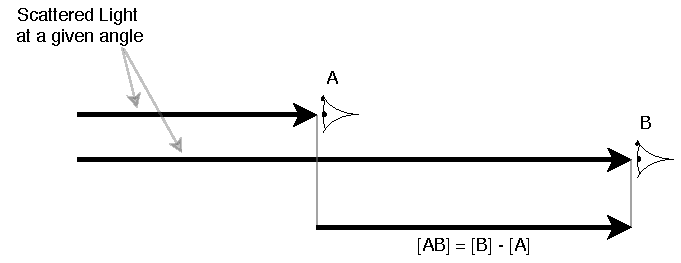
\includegraphics[width=.45\linewidth]{%...
%             img/pdf/spectralMeasurementSketch.pdf}\\
%         \small (a)
%     \end{tabular}
%     \hfill
%     \begin{tabular}[b]{c}
%         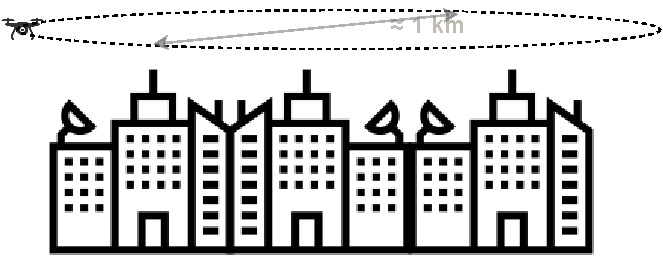
\includegraphics[width=.45\linewidth]{%...
%             img/pdf/spectralMeasurementsFromTheSide.pdf}\\
%         \small (b)
%     \end{tabular}
%     \caption{a) The measurement idea: light absorption between A and B
%     is given by the subtraction of A from B. b) Schematic representation
%     of a measurement operation, side view.}
%     \label{fig:measurement}
% \end{figure}





% \section{The Simulator: TomoSim}%
% \label{sec:the_simulator_tomosim}

% \subsection{Tomographic Procedures}%
% \label{sub:tomographic_procedures}

% As discussed in Subsection~\ref{sub:measurement_trajectory}, the UAV's
% trajectory and acquisition strategy generate what is treated
% subsequently as a fanbeam geometry problem. Before reconstructing the
% spectral image however, one must convert the continuous nature of the
% natural space into a discrete model, which can be interpreted by the
% computer, in the discretisation step. Siddon's algorithm is used for
% this effect. It allows the calculation of the optical path for each ray
% in a fan. More importantly, it returns the portion of these paths that
% is in each "pixel". This is a very important piece of data, since it
% will be assembled onto what is called the system matrix, which
% fundamental for iterative reconstruction methods.

% The most important part of the implementation of Siddon's algorithm in
% what concerns this simulator is the determination of three starting
% parameters: number of lines, line starting point (p1) and line finishing
% point (p2). The first parameter is set by the number of pixels in the
% phantom, which is a configurable parameter. p1 is also in part set by
% the size of the phantom, but also depends on the projection angle. p2 is
% algebrically calculated using the ray's slope to determine its line
% equation and then some vector properties to find where this line
% intersects the trajectory circumference, which becomes a matter of
% solving a simple second degree equation after some algebric
% manipulation. After these three parameters are completely determined,
% discretisation of the field of analysis is achieved through a normal
% implementation of Siddon's algorithm, as is described in
% Section~\ref{sec:theoretical_background}.

% With the space conveniently discretised, the routine starts
% reconstructing the image from the generated projection data. Since no
% actual measurements were conducted during the development of this
% simulation, gas concentration was also simulated, as well as their
% spatial distribution. Concentration values, which actually are column
% density values, were chosen to be similar to the ones that can be found
% in nature. Spatial distribution information is provided to the
% simulation routine in a phantom form. In tomography, a phantom is an
% artificial image that is used to test reconstruction algorithms. One of
% the most commonly used phantoms in tomographic imaging is the
% Shepp-Logan phantom (see Figure~\ref{fig:shepplogan}), which was
% designed to mimic the human head structure. This phantom is very readily
% available in the relevant literature and was therefore used for the
% development of this simulation routine. The phantom's structure,
% however, is not very adequate to one of atmospheric spectral imaging.
% For this reason, the phantom presented in Figure~\ref{fig:new_phantom}
% was designed.

% \begin{figure}
%    \centering 
%    \begin{tabular}[b]{c}
%       
\includegraphics[width=0.45\textwidth]{img/png/shepp_logan.png}\\
%       \small (a)
%    \end{tabular}
%    \hfill
%    \begin{tabular}[b]{c}
%        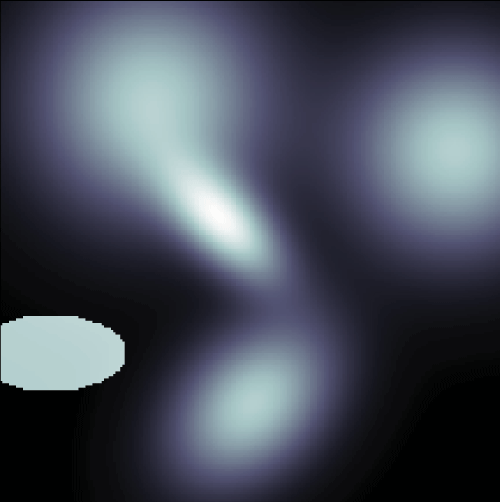
\includegraphics[width=.45\textwidth]{img/png/spectral.png}\label{fig:new_phantom}\\
%       \small (b)
%    \end{tabular}
%    \caption{Set of phantoms used in the TomoSim simualtor: a) the
%    Shepp-Logan phantom, commonly used in medical imaging; b) a new
%    phantom, designed for the tomographic reconstruction of atmospheric
%    gas distribution.}\label{fig:phantoms}
% \end{figure}
% % \begin{figure}
% %     \begin{subfloat}{0.45\textwidth}
% %         \begin{center}
% %             %         \end{center}
% %         \caption{Shepp-Logan phantom, commonly used in medical imaging.}
% %         \label{fig:shepplogan}
% %     \end{subfloat}
% %     \hfill
% %     \begin{subfloat}{0.45\textwidth}
% %         \begin{center}
% %             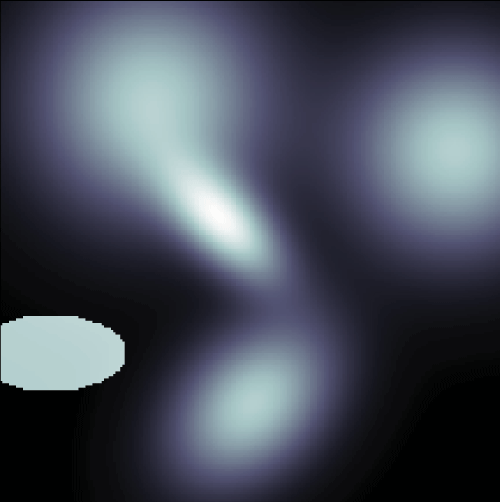
\includegraphics[width=\textwidth]{img/png/spectral.png}
% %         \end{center}
% %         \caption{New phantom, designed for spectroscopic analysis of
% %         atmopsheric trace gases.}
% %         \label{fig:new_phantom}
% %     \end{subfloat}
% %     \caption{Set of phantoms used for the Tomosim simulator.}
% % \end{figure}

% In this simulation, the pixel value is related to the concentration of
% the trace gas being sampled by using the projections themselves as
% normalising units. Light enters the Region Of Interest at point P1 and
% leaves at point P2. At the entrance point, light is simulated through
% the use of a solar spectrum with no atmospheric contamination (see
% ~\cite{Kurucz1984}). The ROI is populated with the some concentration of
% trace gases that one wants to simulate, distributed along one of the
% phantom matrices that have been discussed. Pixel values in these
% matrices are equated to molecule numbers.

% When setup in this manner, one can simulate a detector \emph{looking}
% from point P2 to point P1, and \emph{seeing} the contamination of the
% solar spectrum by the trace gases in the phantom. The simulator then
% applies the Siddon algorithm from P1 to P2 and thus calculates the
% number of molecules traversed by each ray of light. All the numbers for
% all the projections are then assembled onto a single matrix, the
% sinogram. The optical lengths of each pixel for each ray are also stored
% in the system matrix. In real life measurements, this process is
% slightly more complicated, because the contamination at point P1 is not
% known \emph{a priori}.

% Reconstruction algorithms \emph{per se} only start at this point, in two
% ways: iterative and analytical. For the latter, there is still an
% intermediate step, in which the fanbeam sinogram collected by the device
% is transformed into a parallel projection sinogram (pseudocode for this
% transformation is shown in Algorithm~\ref{alg:resorting}). Iterative
% algorithms, however, do not require this step, since they are mostly
% independent of the problem's geometry~\cite{Defrise2003}.

% After running the reconstruction, the simulator already provides a
% twodimensional map of the trace gas in the ROI, but it lacks the numeric
% values for the measured densities. The image matrix is, at this point, a
% collection of 32 bit floating point numbers from 0 to 1. These numbers
% can be normalised by running Siddon's algorithm again for a limited
% number of projections, and equating calculated projections with the ones
% that were acquired from the original phantom.

% \section{The Experiment}%
% \label{sec:the_experiment}

% \begin{figure}[htpb]
%     \centering
%     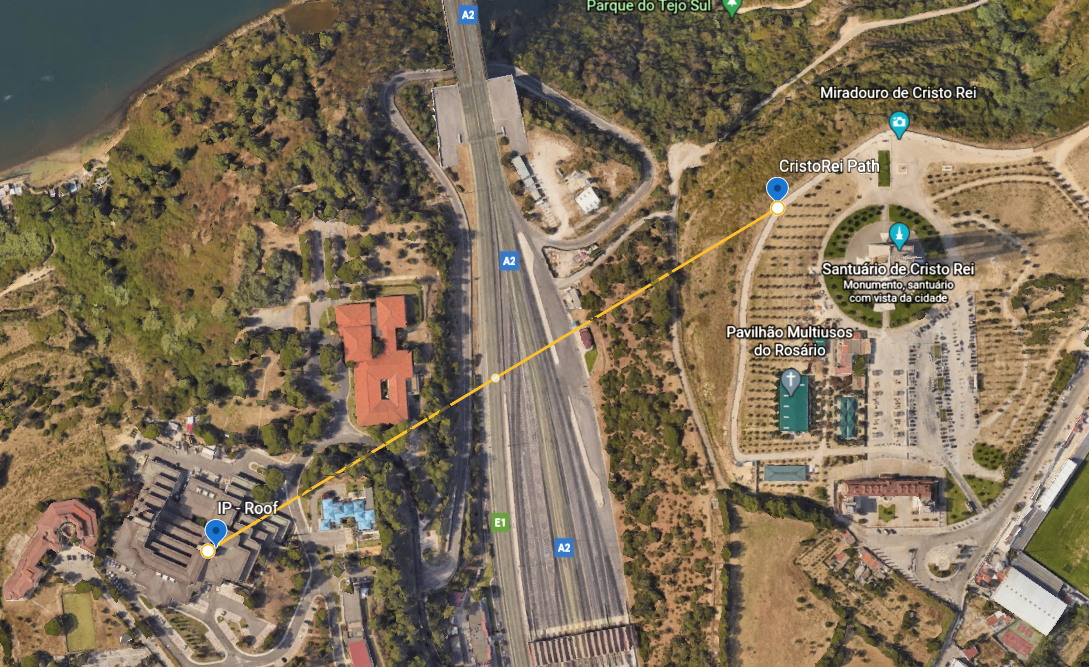
\includegraphics[width=0.8\linewidth]{img/png/experimentMap.png}
%     \caption{Location of observer points for the physical experiment.}
%     \label{fig:experiment_map}
% \end{figure}
